\documentclass[12pt]{article}
\usepackage[utf8]{inputenc}
\usepackage[polish]{babel}
\usepackage[T1]{fontenc}
\usepackage{abstract}
\usepackage{geometry}
\usepackage{graphicx}
\usepackage{hyperref}
\usepackage{amsmath}
\usepackage{float}
\usepackage[backend=bibtex]{biblatex}
\usepackage{csquotes}
\addbibresource{bibliografia.bib}

\geometry{a4paper, left=25mm, right=25mm, top=30mm, bottom=30mm}

\hypersetup{
    colorlinks=false,
    pdfborder={0 0 0},
}

% Nadpisanie tłumaczeń z pakietu babel
\addto\captionspolish{
  \renewcommand{\abstractname}{Abstrakt}
  \renewcommand{\refname}{Bibliografia}
}

\DeclareCiteCommand{\supercite}[\mkbibsuperscript]
  {\iffieldundef{prenote}
     {}
     {\BibliographyWarning{Ignoring prenote argument}}%
   \iffieldundef{postnote}
     {}
     {\BibliographyWarning{Ignoring postnote argument}}}
  {\usebibmacro{citeindex}%
   \bibopenbracket\usebibmacro{cite}\bibclosebracket}
  {\supercitedelim}
  {}

\title{Przegląd ataków adversarialnych na sieci konwolucyjne (CNN)}
\author{
    Wojciech Bartoszek \\
    Łukasz Checiak
}
\date{}

\begin{document}

\maketitle

\begin{center}
    Opiekun:\ prof.\ dr\ hab.\ inż.\ Rafał Scherer
\end{center}

\begin{abstract}
    Sieci konwolucyjne (CNN) zrewolucjonizowały przetwarzanie obrazów, jednak pozostają podatne na ataki adversarialne --- celowo wprowadzone subtelne zakłócenia w danych wejściowych, które wprowadzają błędy w przewidywaniach modeli. W niniejszej pracy eksperymentalnej przeanalizowano metody ataków adversarialnych na CNN, ich skutki oraz strategie obronne. Scharakteryzowano podstawowe techniki takie jak Fast Gradient Sign Method (FGSM), Projected Gradient Descent (PGD), ataki Carliniego-Wagnera oraz DeepFool, ze szczególnym uwzględnieniem ich podstaw matematycznych i skuteczności praktycznej. Przeprowadzono eksperymenty na podzbiorze danych walidacyjnych ImageNet oraz obrazach hiperspektralnych z wykorzystaniem pięciu architektur sieci konwolucyjnych (ResNet50, VGG16, DenseNet121, MobileNetV2, HybridSN). Omówiono mechanizmy obronne, w tym przetwarzanie wstępne danych poprzez kompresję JPEG, wskazując na ich skuteczność w mitigacji ataków adversarialnych. Wykazano uniwersalną podatność architektur CNN na ataki, przy czym ResNet50 wykazuje najwyższą odporność, a ataki Carlini \& Wagner okazują się najskuteczniejsze. Przeanalizowano także efekt kompresji JPEG jako naturalnego mechanizmu defensywnego. Wyniki wskazują na fundamentalne wyzwanie związane z równoważeniem dokładności i odporności modeli oraz konieczność rozwoju wielowarstwowych strategii ochronnych. Zaproponowano kierunki przyszłych badań obejmujące projektowanie inherentnie odpornych architektur oraz zaawansowane metody preprocessing'u defensywnego. Praca integruje perspektywę teoretyczną i praktyczną, oferując kompleksowy obraz wyzwań bezpieczeństwa w głębokich sieciach neuronowych.
\end{abstract}


\section{Wprowadzenie}

Współczesne sieci konwolucyjne (CNN) osiągnęły niezwykłe sukcesy w zadaniach rozpoznawania obrazów, jednak ich podatność na ataki adversarialne stanowi poważne wyzwanie dla bezpieczeństwa systemów opartych na uczeniu maszynowym \supercite{szegedy2013intriguing}. Ataki adversarialne polegają na wprowadzeniu celowych, często niedostrzegalnych dla człowieka, modyfikacji do danych wejściowych, które prowadzą do błędnych przewidywań modelu. Zjawisko to budzi szczególne obawy w kontekście zastosowań krytycznych, takich jak autonomiczne pojazdy, systemy medyczne czy bezpieczeństwo publiczne.

Celem niniejszej pracy jest przeprowadzenie kompleksowej analizy wpływu różnych metod ataków adversarialnych na wydajność wybranych architektur CNN. Badanie koncentruje się na czterech fundamentalnych technikach ataku:

\begin{itemize}
    \item \textbf{FGSM (Fast Gradient Sign Method)} \supercite{goodfellow2014explaining} --- jednokrokowa metoda gradientowa charakteryzująca się wysoką efektywnością obliczeniową
    \item \textbf{PGD (Projected Gradient Descent)} \supercite{madry2017towards} --- iteracyjne rozszerzenie FGSM zapewniające większą skuteczność
    \item \textbf{Carlini \& Wagner (C\&W)} \supercite{carlini2017towards} --- zaawansowany atak optymalizacyjny minimalizujący perturbacje
    \item \textbf{DeepFool} \supercite{moosavi2016deepfool} --- metoda geometryczna znajdująca minimalne zaburzenia prowadzące do zmiany klasyfikacji
\end{itemize}

Analiza empiryczna obejmuje cztery reprezentatywne architektury CNN, charakteryzujące się różnymi podejściami projektowymi:

\begin{itemize}
    \item \textbf{ResNet50} --- architektura wykorzystująca połączenia rezydualne
    \item \textbf{VGG16} --- klasyczna głęboka sieć konwolucyjna
    \item \textbf{DenseNet121} --- architektura z gęstymi połączeniami między warstwami
    \item \textbf{MobileNetV2} --- efektywna obliczeniowo sieć przeznaczona na urządzenia mobilne
\end{itemize}

Eksperymenty przeprowadzono na reprezentatywnym podzbiorze zbioru walidacyjnego ImageNet, zawierającym 128 obrazów z różnych klas, co umożliwia kontrolowaną ocenę odporności modeli przy zachowaniu obliczeniowej wykonalności eksperymentów. Dodatkowo, w celu rozszerzenia zakresu analizy, zbadano także wpływ ataków na obrazy hiperspektralne z wykorzystaniem modelu HybridSN na zbiorze danych Indian Pines, oraz skuteczność kompresji JPEG jako metody defensywnej. Kod źródłowy implementacji oraz szczegółowe wyniki eksperymentów zostały udostępnione publicznie pod adresem: \url{https://github.com/f4rys/Cross-Domain-Adversarial-Analysis}

\section{Metodologia ataków adversarialnych}

W niniejszym badaniu zaimplementowano cztery fundamentalne metody ataków adversarialnych w frameworku PyTorch, wykorzystując specyficzne warianty i optymalizacje dostosowane do charakterystyki badanych modeli. Wszystkie implementacje bazują na oryginalnych algorytmach z literatury, lecz zostały zoptymalizowane pod kątem wydajności obliczeniowej i stabilności numerycznej.

\subsection{Fast Gradient Sign Method (FGSM)}

Fast Gradient Sign Method \supercite{goodfellow2014explaining} stanowi fundament jednokrokowych ataków adversarialnych. W eksperymentach wykorzystano wariant $untargeted$, który maksymalizuje funkcję straty dla prawdziwej etykiety bez określania konkretnej klasy docelowej. Implementacja wykorzystuje CrossEntropyLoss i wykonuje gradient ascent względem danych wejściowych.

Matematycznie, adversarialny przykład $x'$ generowany jest zgodnie z równaniem:

\begin{equation}
    x' = x + \epsilon \cdot \text{sign}(\nabla_x J(\theta, x, y))
\end{equation}

gdzie $x$ oznacza oryginalny obraz, $\epsilon$ parametr kontrolujący intensywność ataku. $J(\theta, x, y)$ funkcję straty modelu z parametrami $\theta$ dla danej pary (obraz, etykieta), a $\nabla_x J$ gradient tej funkcji względem danych wejściowych.

Główną zaletą FGSM jest jego efektywność obliczeniowa --- wymaga jedynie jednokrotnego obliczenia gradientu.

\subsection{Projected Gradient Descent (PGD)}

Projected Gradient Descent \supercite{madry2017towards} stanowi iteracyjne rozszerzenie metody FGSM, zaimplementowane jako wariant $untargeted$ z normą $\ell_\infty$. Algorytm wykonuje wielokrotną aktualizację perturbacji z projekcją na kulę $\ell_\infty$ o promieniu $\epsilon$.

Algorytm PGD można sformalizować jako:

\begin{equation}
    x^{t+1} = \Pi_{S}(x^t + \alpha \cdot \text{sign}(\nabla_x J(\theta, x^t, y)))
\end{equation}

gdzie $\Pi_{S}$ oznacza operację projekcji na dopuszczalny zbiór perturbacji $S$ (kulę $\ell_\infty$ o promieniu $\epsilon$), $\alpha$ rozmiar kroku, a $t$ numer iteracji.

Implementacja zawiera mechanizm wczesnego zatrzymywania --- jeśli gradient względem obrazu adversarialnego wynosi zero (co może oznaczać maksymalne błędne przewidywanie), algorytm przerywa iteracje dla danej próbki.

\subsection{Carlini \& Wagner (C\&W)}

Atak Carlini \& Wagner \supercite{carlini2017towards} reprezentuje zaawansowane podejście optymalizacyjne zaimplementowane jako wariant $untargeted$ z normą $\ell_2$. W przeciwieństwie do metod gradientowych, C\&W formułuje problem jako zadanie optymalizacji z ograniczeniami wykorzystując AdamW optimizer.

Implementacja wykorzystuje transformację atanh dla zapewnienia, że wartości pikseli pozostają w dopuszczalnym zakresie:

\begin{equation}
    x' = \frac{1}{2}(\tanh(w) + 1), \quad w = \text{atanh}(2x - 1)
\end{equation}

Funkcja celu łączy stratę klasyfikacyjną z regularyzacją $\ell_2$:

\begin{equation}
    \min \|x' - x\|_2 + c \cdot f(x')
\end{equation}

gdzie $f(x') = \max(Z(x')_{y} - \max_{j \neq y} Z(x')_j + \kappa, 0)$ z $Z(x')$ oznaczającym logity.

Implementacja zawiera mechanizm $best-candidate tracking$ --- przechowuje najlepsze adversarialne przykłady (o najmniejszej normie $\ell_2$) spośród tych, które skutecznie wprowadzają błędną klasyfikację.

\subsection{DeepFool}

DeepFool \supercite{moosavi2016deepfool} wykorzystuje geometryczne podejście implementowane jako wariant $untargeted$ minimalizujący normę $\ell_2$. Algorytm iteracyjnie aproksymuje granice decyzyjne klasyfikatora poprzez znajdowanie najbliższej hiperpłaszczyzny separującej klasy.

Implementacja wykorzystuje obliczenia macierzy Jacobian dla efektywnego wyliczenia gradientów względem wszystkich klas jednocześnie. W każdej iteracji $t$, DeepFool oblicza minimalną perturbację $r_t$ potrzebną do przekroczenia lokalnej granicy decyzyjnej:

\begin{equation}
    r_t = \frac{|f_k(x_t) - f_{j^*}(x_t)|}{\|\nabla f_k(x_t) - \nabla f_{j^*}(x_t)\|_2^2} (\nabla f_k(x_t) - \nabla f_{j^*}(x_t))
\end{equation}

gdzie $j^*$ oznacza klasę znajdującą się najbliżej granicy decyzyjnej, $f_k$ różnicę logitów między klasą aktualnie przewidywaną a klasą $k$.

\section{Architektury sieci neuronowych}

W niniejszym badaniu wykorzystano cztery reprezentatywne architektury CNN oraz jedną architekturę dedykowaną obrazom hiperspektralnym. Każda z nich charakteryzuje się odmiennym podejściem projektowym i różnymi mechanizmami uczenia. Wybór tych modeli pozwala na kompleksową ocenę wpływu różnych strategii architekturalnych na odporność względem ataków adversarialnych.

\begin{itemize}
    \item \textbf{ResNet50} \supercite{he2016deep} --- architektura wprowadzająca koncepcję połączeń rezydualnych (skip connections), które umożliwiają trenowanie bardzo głębokich sieci poprzez rozwiązanie problemu zaniku gradientu. Połączenia te pozwalają na bezpośredni przepływ informacji między odległymi warstwami, co teoretycznie może wpływać na odporność modelu na perturbacje adversarialne.
    \item \textbf{VGG16} \supercite{simonyan2014very} --- klasyczna architektura charakteryzująca się prostą, sekwencyjną strukturą złożoną z małych filtrów konwolucyjnych (3×3). Mimo swojej prostoty, VGG16 pozostaje ważnym punktem odniesienia w badaniach nad sieciami konwolucyjnymi oraz stanowi reprezentację tradycyjnych podejść architekturalnych.
    \item \textbf{DenseNet121} \supercite{huang2017densely} --- sieć wykorzystująca gęste połączenia, w której każda warstwa otrzymuje informacje ze wszystkich poprzedzających warstw. Taka architektura promuje ponowne wykorzystanie cech (feature reuse) i może prowadzić do lepszej regularyzacji, co potencjalnie wpływa na odporność adversarialną.
    \item \textbf{MobileNetV2} \supercite{sandler2018mobilenetv2} --- efektywna obliczeniowo architektura zaprojektowana z myślą o urządzeniach o ograniczonych zasobach. Wykorzystuje separowalne konwolucje depthwise oraz połączenia rezydualne w blokach z wąskim gardłem (inverted residuals), co znacząco redukuje liczbę parametrów.    
    \item \textbf{HybridSN} \supercite{roy2019hybridsn} --- specjalistyczna architektura przeznaczona do klasyfikacji obrazów hiperspektralnych. Model ten wykorzystuje hybrydowe podejście, łącząc konwolucje 3D (do ekstrakcji cech spektralno-przestrzennych) z konwolucjami 2D (do dalszej ekstrakcji cech przestrzennych). Taka hierarchiczna struktura pozwala na efektywne przetwarzanie danych hiperspektralnych o wysokiej wymiarowości.
\end{itemize}

Wszystkie modele CNN zostały wczytane jako przedtrenowane wersje z biblioteki torchvision, przeszkolone na pełnym zbiorze danych ImageNet. W niniejszych eksperymentach wykorzystano implementację modelu HybridSN opartą na PyTorch oraz przedtrenowane wagi dostępne w repozytorium GitHub \supercite{hybridsn_implementation}. W eksperymentach wykorzystano reprezentatywny podzbiór 128 obrazów z różnych klas ze zbioru walidacyjnego ImageNet dla modeli CNN, oraz 8192 próbek z 16 klas dla modelu HybridSN na zbiorze Indian Pines, co umożliwia kontrolowaną ocenę odporności modeli przy zachowaniu obliczeniowej wykonalności eksperymentów. Przed przystąpieniem do ataków adversarialnych dokonano oceny baseline'owej dokładności na wybranych podzbiorach.

\section{Metodologia eksperymentalna i wyniki}

\subsection{Konfiguracja eksperymentów}

Wszystkie eksperymenty zostały przeprowadzone w środowisku PyTorch z wykorzystaniem GPU NVIDIA dla przyspieszenia obliczeń. Dla zapewnienia powtarzalności wyników, ziarno losowości zostało ustalone na stałą wartość. Każdy model był poddawany atakom w odrębnych sesjach w celu uniknięcia interferencji między eksperymentami.

Parametry ataków zostały ustalone następująco: $\epsilon = 0.03$ dla ataków FGSM i PGD, liczba iteracji PGD = 1, rozmiar kroku $\alpha = 0.005$. Dla ataku C\&W wykorzystano parametr confidence $\kappa = 0$ oraz maksymalnie 5 iteracji optymalizacji oraz parametrem $c=5$. DeepFool był uruchamiany z maksymalnie 5 iteracjami oraz parametrem $overshoot=0.05$.

\subsection{Wyniki ataków na klasyfikację obrazów}

Ocena wpływu ataków adversarialnych została przeprowadzona poprzez pomiar dokładności klasyfikacji przed i po zastosowaniu perturbacji. Wyniki przedstawione na Rysunku \ref{fig:model-comparison} oraz w Tabeli \ref{tab:attack-results} ujawniają znaczące różnice w odporności poszczególnych architektur.
\begin{figure}[H]
    \centering
    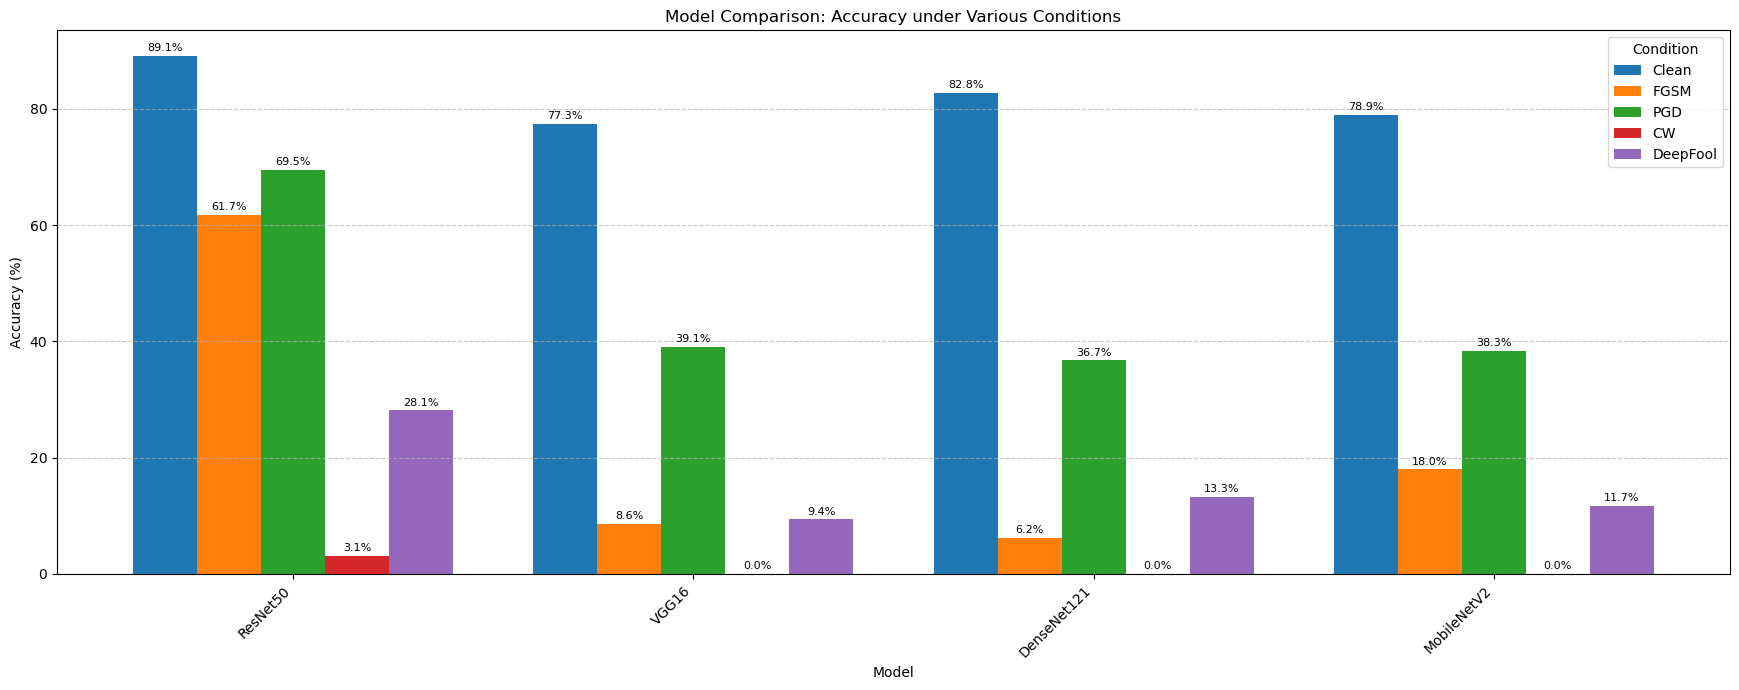
\includegraphics[width=1\textwidth]{model_comparison.png}
    \caption{Wpływ różnych ataków adversarialnych na dokładność klasyfikacji poszczególnych architektur CNN}
    \label{fig:model-comparison}
\end{figure}

\begin{table}[H]
    \centering
    \begin{tabular}{|l|c|c|c|c|c|}
    \hline
    \textbf{Model} & \textbf{Clean} & \textbf{FGSM} & \textbf{PGD} & \textbf{C\&W} & \textbf{DeepFool} \\
    \hline
    ResNet50 & 89.06\% & 61.72\% & 69.53\% & 3.12\% & 28.12\% \\
    VGG16 & 77.34\% & 8.59\% & 39.06\% & 0.00\% & 9.38\% \\
    DenseNet121 & 82.81\% & 6.25\% & 36.72\% & 0.00\% & 13.28\% \\
    MobileNetV2 & 78.91\% & 17.97\% & 38.28\% & 0.00\% & 11.72\% \\
    \hline
    \end{tabular}
    \caption{Dokładność klasyfikacji poszczególnych modeli przed i po zastosowaniu ataków adversarialnych}
    \label{tab:attack-results}
\end{table}

Analiza przedstawionych rezultatów ujawnia znaczące różnice w podatności badanych architektur. ResNet50 wykazuje najwyższą odporność na większość typów ataków, co może być związane z mechanizmem połączeń rezydualnych ułatwiającym gradientowy przepływ informacji. W przeciwieństwie do tego, architektura VGG16 okazuje się być najbardziej podatna, szczególnie w przypadku ataku FGSM, gdzie dokładność spada do zaledwie 8.59\%.

Szczególnie istotnym obserwacjom podlega uniwersalna skuteczność ataku C\&W, który powoduje niemal całkowitą degradację wydajności wszystkich testowanych modeli. Wynik ten potwierdza przewagę metod optymalizacyjnych nad jednokrokowymi atakami gradientowymi w kontekście znajdowania minimalnych perturbacji adversarialnych.

\begin{figure}[H]
    \centering
    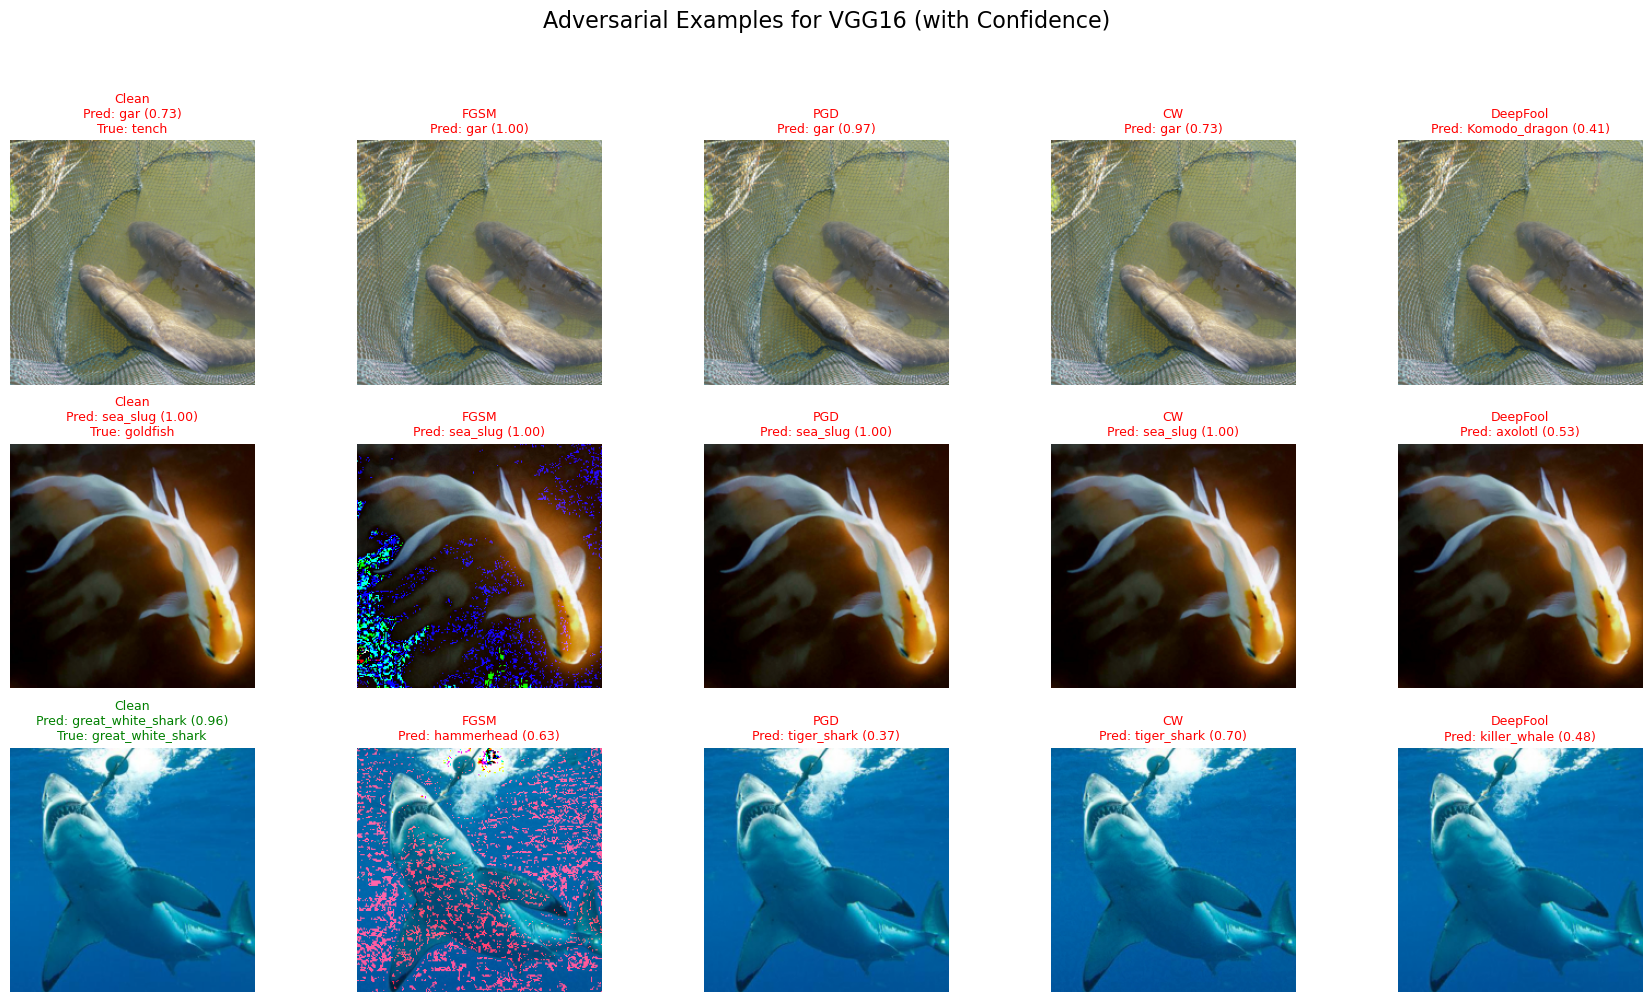
\includegraphics[width=1\textwidth]{adversarial_examples.png}
    \caption{Porównanie wizualnej percepcji oryginalnych obrazów i ich adversarialnych odpowiedników}
    \label{fig:adversarial-examples}
\end{figure}

Analiza wizualna przedstawionych przykładów adversarialnych (Rysunek \ref{fig:adversarial-examples}) ujawnia fundamentalną właściwość tego typu ataków --- ich subtelność względem ludzkiej percepcji. Podczas gdy perturbacje wprowadzone przez atak FGSM są wizualnie dostrzegalne jako zwiększony szum w obrazie, modyfikacje wynikające z zastosowania PGD, C\&W oraz DeepFool pozostają praktycznie niewidoczne dla ludzkiego oka.

Ta obserwacja ma kluczowe znaczenie dla bezpieczeństwa systemów wizyjnych, ponieważ wskazuje na możliwość wprowadzenia złośliwych modyfikacji do obrazów bez wzbudzenia podejrzeń u operatorów lub użytkowników końcowych. Szczególnie problematyczne jest to w kontekście zastosowań krytycznych, gdzie decyzje podejmowane przez systemy CNN mogą mieć bezpośredni wpływ na bezpieczeństwo lub zdrowie.
\subsection{Analiza ataków na dane hiperspektralne}

Obrazy hiperspektralne charakteryzują się znacznie większą złożonością informacyjną w porównaniu do konwencjonalnych obrazów RGB, zawierając setki pasm spektralnych dla każdego piksela. Ta właściwość czyni je szczególnie wartościowymi w zastosowaniach takich jak teledetekcja, monitoring środowiskowy, czy analiza medyczna, ale jednocześnie stwarza nowe wyzwania w kontekście ataków adversarialnych.

W niniejszym badaniu zastosowano architekturę HybridSN \supercite{roy2019hybridsn}, specjalnie zaprojektowaną do klasyfikacji obrazów hiperspektralnych poprzez kombinację konwolucji 3D i 2D. Model ten wykorzystuje zarówno informacje przestrzenne jak i spektralne, co teoretycznie może wpływać na jego odporność względem perturbacji adversarialnych.

W celu zapewnienia stabilności eksperymentów na danych hiperspektralnych, parametry ataków zostały skalibrowane na niższe wartości w porównaniu do eksperymentów na obrazach ImageNet: FGSM z $\epsilon = 0{,}01$, PGD z $\epsilon = 0{,}01$, $\alpha = 0{,}003$ i 1 iteracją, C\&W z parametrem $c = 100$, $\kappa = 0$, 20 iteracjami i learning rate $0{,}05$, oraz DeepFool z 1 iteracją i parametrem overshoot $0{,}01$. Mimo zastosowania słabszych parametrów ataków, model HybridSN wykazał znacznie większą podatność niż CNN testowane na ImageNet z silniejszymi parametrami.

\begin{figure}[H]
    \centering
    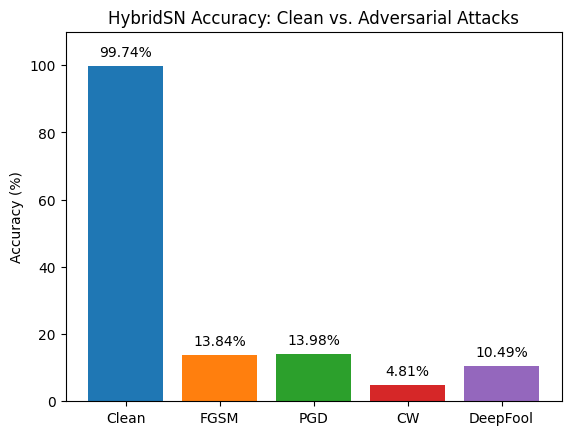
\includegraphics[width=1\textwidth]{hybridsn_accuracy.png} 
    \caption{Dokładność klasyfikacji obrazów hiperspektralnych po zastosowaniu różnych typów ataków adversarialnych}
    \label{fig:hyperspectral-accuracy}
\end{figure}

Wyniki przedstawione na Rysunku \ref{fig:hyperspectral-accuracy} ujawniają znaczące różnice w odporności modelu HybridSN na ataki adversarialne w porównaniu do konwencjonalnych architektur CNN. Wszystkie badane ataki degradują skuteczność HybridSN w większym stopniu niż jakąkolwiek z badanych architektur CNN, co stanowi istotną obserwację dla bezpieczeństwa systemów klasyfikacji hiperspektralnej.

Ta zwiększona podatność HybridSN może wynikać z architekturalnych czynników:

\begin{itemize}
    \item \textbf{Prostota architektury} --- HybridSN wykorzystuje stosunkowo prostą kombinację warstw konwolucyjnych 3D i 2D bez zaawansowanych mechanizmów regularyzacyjnych obecnych w nowoczesnych CNN, takich jak połączenia rezydualne w ResNet50 czy normalizacja batch.
    
    \item \textbf{Mniejsza głębokość sieci} --- W porównaniu do głębokich architektur CNN (ResNet50: 50 warstw, DenseNet121: 121 warstw), HybridSN charakteryzuje się znacznie mniejszą liczbą warstw, co może ograniczać jego zdolność do uczenia się odpornych reprezentacji.
\end{itemize}

\begin{figure}[H]
    \centering
    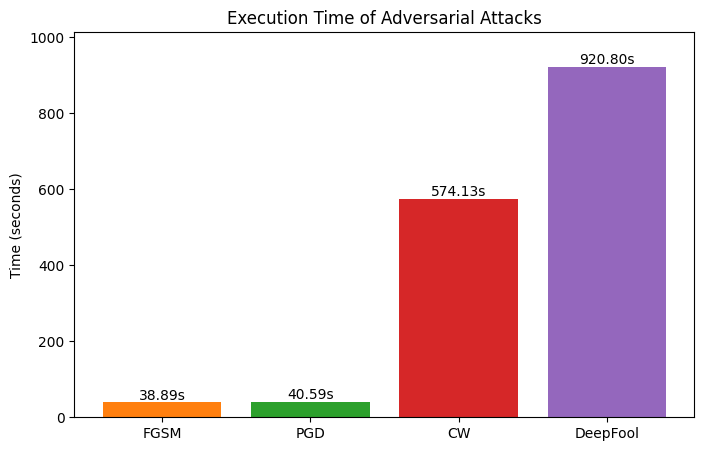
\includegraphics[width=1\textwidth]{hybridsn_time.png} 
    \caption{Analiza czasowa wykonania ataków adversarialnych na dane hiperspektralne}
    \label{fig:hyperspectral-time}
\end{figure}

Analiza efektywności obliczeniowej (Rysunek \ref{fig:hyperspectral-time}) ujawnia wyraźny podział ataków na dwie kategorie. Metody gradientowe (FGSM, PGD) charakteryzują się wysoką efektywnością czasową, wykonując się w czasie około 40 sekund. W przeciwieństwie do tego, ataki optymalizacyjne (C\&W, DeepFool) wymagają znacznie większych zasobów obliczeniowych, z czasami wykonania sięgającymi odpowiednio około 10 i 15 minut.

\begin{figure}[H]
    \centering
    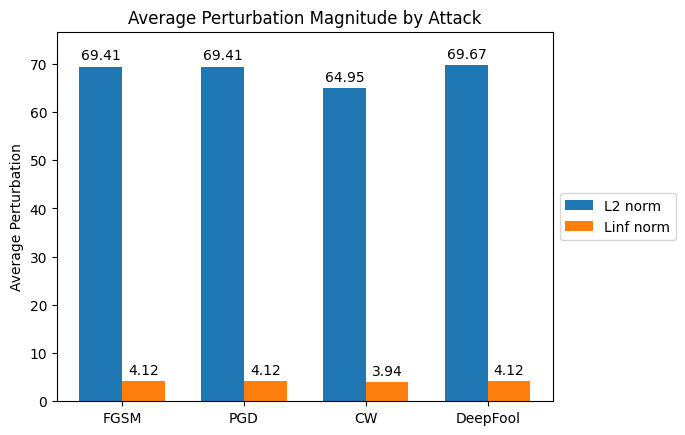
\includegraphics[width=1\textwidth]{perturbations.png} 
    \caption{Porównanie magnitud perturbacji adversarialnych mierzonych normami $\ell_2$ i $\ell_\infty$}
\end{figure}

Analiza magnitud perturbacji została przeprowadzona w celu weryfikacji, czy parametry poszczególnych ataków zostały dobrane tak, aby siła generowanych zaburzeń była porównywalna, co jest warunkiem koniecznym dla rzetelnej oceny ich skuteczności. W analizie wykorzystano dwie fundamentalne normy:
\begin{itemize}
    \item norma $\ell_2$ - mierzy całkowitą energię zaburzenia, czyli jego długość w przestrzeni euklidesowej. W praktyce oznacza to, że jeśli zaburzenie jest rozproszone równomiernie po wielu pikselach i pasmach spektralnych, ale o małej sile, to norma $\ell_2$ będzie niska. Jest to często stosowane do oceny subtelnych, „gładkich” perturbacji.
    \item norma $\ell_\infty$ - mierzy maksymalną zmianę wartości w jednym pikselu. Określa więc, jak bardzo zaburzenie może zmienić dowolną pojedynczą wartość w obrazie. Tę normę stosuje się, gdy celem jest ograniczenie „najgorszego przypadku” zmiany, nawet jeśli cała reszta obrazu pozostaje praktycznie nietknięta.
\end{itemize}
Wartości uzyskane są bardzo podobne, norma $\ell_2$ dla C\&W jest trochę mniejsza, co może sugerować, że potrzebna była mniejsza czułość do skutecznego przeprowadzenia ataku. Uzyskane wyniki raczej pokazują odporność samego zbioru danych na ataki, niż skuteczność ich samą w sobie. Ogólnie więc możemy ten wykres interpretować tak, że potrzebne było dość duże zaburzenie globalne (norma $\ell_2$) oraz że zmiana lokalna (maksymalna dla pojedynczego piksela) może być widoczna, jednak raczej dla obrazów o niższej rozdzielczości ($\ell_\infty$).

\subsection{Wpływ kompresji JPEG na skuteczność ataków adversarialnych}

\begin{figure}[H]
    \centering
    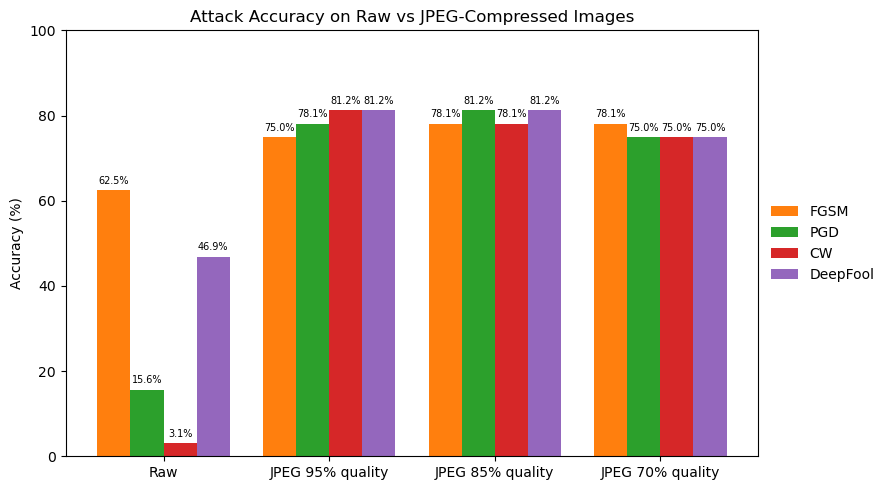
\includegraphics[width=1\textwidth]{jpeg_accuracy.png}
    \caption{Wpływ kompresji JPEG na skuteczność ataków adversarialnych w architekturze ResNet50}
    \label{fig:jpeg-compression}
\end{figure}

Kompresja JPEG stanowi powszechnie stosowaną metodę redukcji rozmiaru plików obrazowych poprzez eliminację wysokoczęstotliwościowych składowych sygnału. W kontekście ataków adversarialnych, proces ten może nieintencjonalnie działać jako mechanizm defensywny poprzez usunięcie perturbacji zakodowanych w wysokich częstotliwościach przestrzennych.

Analiza ujawnia znaczący wpływ kompresji JPEG na mitigację ataków adversarialnych. Po zastosowaniu kompresji stratnej, dokładność klasyfikacji wzrosła do poziomu około 80\% dla wszystkich typów ataków, co w przypadku ataku C\&W oznacza spektakularny wzrost o 77 punktów procentowych w porównaniu do 3\% dokładności przed kompresją.

Ten fenomen można wytłumaczyć dwoma fundamentalnymi mechanizmami:

\begin{itemize}
    \item \textbf{Eliminacja wysokoczęstotliwościowych artefaktów} --- algorytm JPEG usuwa komponenty o wysokich częstotliwościach przestrzennych, które często zawierają perturbacje adversarialne generowane przez ataki takie jak FGSM czy PGD.
    
    \item \textbf{Efekt wygładzania} --- proces kwantyzacji i kompresji wprowadza naturalne wygładzenie obrazu, co może osłabiać lokalne perturbacje adversarialne poprzez ich rozmycie w otaczającym kontekście przestrzennym.
\end{itemize}

Należy jednak podkreślić, że kompresja JPEG jako metoda defensywna ma istotne ograniczenia. Po pierwsze, jest to transformacja stratna, co może negatywnie wpływać na jakość danych wejściowych. Po drugie, zaawansowane ataki mogą być dostosowane do odporności na tego typu preprocessing, co potencjalnie mogłoby zniwelować obserwowany efekt defensywny.

\section{Analiza wyników}

Z przedstawionych wyników wynika, że skuteczność ataków adversarialnych znacząco różni się w zależności od użytego modelu i rodzaju ataku. Najważniejsze obserwacje to:

\begin{itemize}
    \item \textbf{ResNet50} wykazuje największą odporność na większość ataków. Dla ataku PGD dokładność spadła do 69{,}5\%, co nadal jest relatywnie wysokim wynikiem w porównaniu do innych modeli. Również przy ataku FGSM ResNet50 zachowuje stosunkowo dobrą skuteczność (61{,}7\%).
    
    \item \textbf{Atak Carlini \& Wagner (C\&W)} okazał się najskuteczniejszy --- doprowadził do niemal całkowitej dezintegracji wszystkich modeli (dokładność od 0\% do 3{,}1\%). Świadczy to o jego precyzyjnej konstrukcji i zdolności do tworzenia zaburzeń minimalnie wpływających na percepcję wizualną, ale bardzo skutecznych wobec klasyfikatorów.
    
    \item \textbf{Modele VGG16, DenseNet121 oraz MobileNetV2} cechuje znacznie niższa odporność na ataki w porównaniu do ResNet50. VGG16, na przykład, osiąga zaledwie 8{,}6\% dokładności przy ataku FGSM i całkowicie zawodzi przy ataku C\&W.
    
    \item \textbf{DeepFool} osiąga umiarkowaną skuteczność — dokładność po ataku waha się od 9{,}4\% do 28{,}1\%. Ciekawym spostrzeżeniem jest jego wizualna subtelność, mimo że potrafi znacząco zaburzyć klasyfikację.
    
    \item \textbf{Hiperspektralne ataki} wykazały podobne właściwości — ataki C\&W ponownie były najskuteczniejsze, co potwierdza ich uniwersalność. Natomiast czas ich wykonania oraz poziom wymaganych zaburzeń wskazują na kompromis pomiędzy skutecznością a kosztami obliczeniowymi.
    
    \item \textbf{Kompresja JPEG} okazuje się być interesującą metodą obrony — znacząco redukuje wpływ ataku, szczególnie dla C\&W, gdzie dokładność wzrosła z 3{,}1\% do około 80\%. Oznacza to, że nawet proste techniki przetwarzania obrazu mogą w pewnych przypadkach niwelować efekty perturbacji.
\end{itemize}

\section{Podsumowanie i wnioski}

Przeprowadzone badania eksperymentalne dostarczają kompleksowego obrazu podatności współczesnych architektur CNN na różne typy ataków adversarialnych. Analiza obejmująca cztery reprezentatywne architektury (ResNet50, VGG16, DenseNet121, MobileNetV2) oraz cztery fundamentalne metody ataków (FGSM, PGD, C\&W, DeepFool) pozwala na sformułowanie następujących kluczowych wniosków:

\subsection{Architekturalne determinanty odporności adversarialnej}

Wyniki eksperymentów jednoznacznie wskazują na znaczące różnice w odporności poszczególnych architektur CNN na ataki adversarialne. \textbf{ResNet50} wykazuje najwyższą odporność spośród badanych modeli, co można przypisać mechanizmowi połączeń rezydualnych ułatwiających stabilny przepływ gradientów i potencjalnie zwiększających regularność przestrzeni reprezentacji. W przeciwieństwie do tego, \textbf{VGG16} okazuje się najbardziej podatny na perturbacje, co może wynikać z jego prostej, sekwencyjnej architektury pozbawionej mechanizmów regularyzacyjnych obecnych w nowszych projektach.

\subsection{Hierarchia skuteczności ataków adversarialnych}

Analiza porównawcza różnych metod ataków ujawnia wyraźną hierarchię ich skuteczności:

\begin{enumerate}
    \item \textbf{Carlini \& Wagner (C\&W)} --- najskuteczniejszy atak we wszystkich scenariuszach, osiągający niemal zerową dokładność klasyfikacji dla wszystkich testowanych architektur. Jego przewaga wynika z zaawansowanego podejścia optymalizacyjnego minimalizującego perturbacje przy maksymalizacji skuteczności.
    
    \item \textbf{DeepFool} --- druga w kolejności skuteczność, wykorzystująca geometryczne podejście do znajdowania minimalnych perturbacji względem granic decyzyjnych.
    
    \item \textbf{PGD} --- iteracyjne rozszerzenie FGSM wykazujące umiarkowaną skuteczność, szczególnie przeciwko modelom o większej odporności jak ResNet50.
    
    \item \textbf{FGSM} --- jednokrokowa metoda o najniższej skuteczności, ale najwyższej efektywności obliczeniowej.
\end{enumerate}

\subsection{Implikacje dla bezpieczeństwa systemów wizyjnych}

Obserwowana subtelność wizualna perturbacji adversarialnych, szczególnie w przypadku ataków C\&W i DeepFool, stwarza poważne zagrożenie dla bezpieczeństwa systemów opartych na CNN. Możliwość wprowadzenia niepostrzegalnych modyfikacji powodujących błędne klasyfikacje ma krytyczne znaczenie w zastosowaniach takich jak:

\begin{itemize}
    \item Systemy autonomicznych pojazdów
    \item Diagnostyka medyczna oparta na analizie obrazów
    \item Systemy bezpieczeństwa i nadzoru
    \item Aplikacje rozpoznawania biometrycznego
\end{itemize}

\subsection{Podatność danych hiperspektralnych}

Rozszerzenie analizy na obrazy hiperspektralne potwierdza uniwersalność problemu ataków adversarialnych niezależnie od modalności danych. Architektura HybridSN, mimo swojej specjalizacji w przetwarzaniu informacji spektralno-przestrzennych, wykazuje podobną podatność na ataki jak konwencjonalne CNN. Ta obserwacja ma szczególne znaczenie dla zastosowań w teledetekcji, monitoringu środowiskowym oraz analizie materiałów.

\subsection{Potencjał metod defensywnych}

Badanie wpływu kompresji JPEG jako nieintencjonalnej metody defensywnej ujawnia obiecujący kierunek rozwoju mechanizmów ochronnych. Spektakularny wzrost dokładności klasyfikacji po kompresji (z 3\% do 80\% dla ataku C\&W) wskazuje na potencjał prostych metod preprocessing'u w mitigacji ataków adversarialnych. Jednakże, należy uwzględnić ograniczenia tej metody, w tym degradację jakości obrazu oraz możliwość adaptacji ataków do odporności na kompresję.

\subsection{Rekomendacje dla przyszłych badań}

Na podstawie przeprowadzonej analizy można wskazać następujące kierunki dalszych badań:

\begin{enumerate}
    \item \textbf{Rozwój architektur inherentnie odpornych} --- projektowanie sieci neuronowych z wbudowanymi mechanizmami odporności na ataki adversarialne.
    
    \item \textbf{Zaawansowane metody preprocessing'u defensywnego} --- eksploracja różnych technik transformacji obrazów jako metod ochronnych.
    
    \item \textbf{Teoretyczne podstawy transferowalności ataków} --- głębsze zrozumienie mechanizmów przenoszenia perturbacji między różnymi architekturami.
    
    \item \textbf{Standaryzacja metodologii oceny} --- opracowanie ujednoliconych benchmarków dla oceny odporności adversarialnej.
    
    \item \textbf{Ataki adaptacyjne} --- badanie ataków dostosowanych do konkretnych mechanizmów defensywnych.
\end{enumerate}

Podsumowując, wyniki niniejszego badania podkreślają fundamentalne wyzwanie jakim są ataki adversarialne dla współczesnych systemów uczenia głębokiego. Skuteczna ochrona przed tego typu zagrożeniami wymaga wielowymiarowego podejścia łączącego zaawansowane architektury, metody treningu adversarialnego oraz preprocessing defensywny. Jednocześnie, ciągła ewolucja technik ataku wymaga stałego rozwoju i adaptacji mechanizmów obronnych.

\printbibliography

\end{document}